% Copyright 2004 by Till Tantau <tantau@users.sourceforge.net>.
%
% In principle, this file can be redistributed and/or modified under
% the terms of the GNU Public License, version 2.
%
% However, this file is supposed to be a template to be modified
% for your own needs. For this reason, if you use this file as a
% template and not specifically distribute it as part of a another
% package/program, I grant the extra permission to freely copy and
% modify this file as you see fit and even to delete this copyright
% notice.
% Adapted by Len Goff, 2019

\documentclass[10pt]{beamer}

% There are many different themes available for Beamer. A comprehensive
% list with examples is given here:
% http://deic.uab.es/~iblanes/beamer_gallery/index_by_theme.html
% You can uncomment the themes below if you would like to use a different
% one:
%\usetheme{AnnArbor}
%\usetheme{Antibes}
%\usetheme{Bergen}
%\usetheme{Berkeley}
%\usetheme{Berlin}
%\usetheme{Boadilla}
%\usetheme{boxes}
%\usetheme{CambridgeUS}
\usetheme{Copenhagen}
%\usetheme{Darmstadt}
%\usetheme{default}
%\usetheme{Frankfurt}
%\usetheme{Goettingen}
%\usetheme{Hannover}
%\usetheme{Ilmenau}
%\usetheme{JuanLesPins}
%\usetheme{Luebeck}
% \usetheme{Madrid}
%\usetheme{Malmoe}
%\usetheme{Marburg}
%\usetheme{Montpellier}
%\usetheme{PaloAlto}
%\usetheme{Pittsburgh}
%\usetheme{Rochester}
%\usetheme{Singapore}
%\usetheme{Szeged}
%\usetheme{Warsaw}

%Some code to format a hyperlink button
\setbeamertemplate{button}{\tikz[baseline={(0,-3.5pt)}]
    \node[
    inner xsep=5pt,
    inner ysep=1pt,
    draw=structure!80,
    fill=structure!50,
    rounded corners=4pt]  {\topskip0pt \normalsize\insertbuttontext};}

%Some packages that will be useful
\usepackage{pgfplots}
\usepackage{cancel}
\usepackage{caption}
\usepackage{dcolumn}
\usepackage{mathtools}
\captionsetup{belowskip=-15pt,aboveskip=0pt}

\def\checkmark{\tikz\fill[scale=0.4](0,.35) -- (.25,0) -- (1,.7) -- (.25,.15) -- cycle;}


\usepackage{sansmathaccent}
\pdfmapfile{+sansmathaccent.map}

\usenavigationsymbolstemplate{}

\usepackage{array}
\newcolumntype{H}{>{\setbox0=\hbox\bgroup}c<{\egroup}@{}}
\usepackage{makecell}

\makeatletter
\def\thmhead@plain#1#2#3{%
    \thm@notefont{}% same as heading font
    \thmname{#1}\thmnumber{\@ifnotempty{#1}{ }\@upn{#2}}%
    \thmnote{ {\the\thm@notefont#3}}}
\let\thmhead\thmhead@plain
\itshape % body font
\makeatother

%Define normal density function for use in tikzpicture
\pgfmathdeclarefunction{gauss}{2}{%
    \pgfmathparse{3/(#2*sqrt(2*pi))*exp(-((x-#1)^2)/(2*#2^2))}%
}


%This allows adjustable spacing in itemize environment
\newenvironment{wideitemize}{\itemize\addtolength{\itemsep}{10pt}}{\enditemize}

%This allows slide numberering to not includethe title slide
\addtocounter{framenumber}{-1}
\addtobeamertemplate{navigation symbols}{}{%
    \usebeamerfont{footline}%
    \usebeamercolor[fg]{footline}%
    \hspace{1em}%
    %uncomment the below if you want frame numbers inside slide rather than in footline
    %\insertframenumber/\inserttotalframenumber
}

%
\newcommand{\backupbegin}{
    \newcounter{finalframe}
    \setcounter{finalframe}{\value{framenumber}}
}
\newcommand{\backupend}{
    \setcounter{framenumber}{\value{finalframe}}
}

\usetikzlibrary{decorations.pathreplacing,angles,quotes}
\usetikzlibrary{patterns}
\usetikzlibrary{positioning}
\usetikzlibrary{decorations.text}
\usetikzlibrary{decorations.pathmorphing}

%\title{Entangled instrumental variables}
\title{Banking the unbanked}
\subtitle{Future-proofing the least developed countries as they go from cash to online payment}

% A subtitle is optional and this may be deleted
%\subtitle{Optional Subtitle}

\author{Martin Thiele}

\institute[University of Copenhagen] % (optional, but mostly needed)
{
    Master's Thesis\\June 17, 2021\\
    \bigskip \bigskip mqn507@alumni.ku.dk
}

\date{}

\usepackage{graphicx}
\usepackage{bbm}

\graphicspath{ {images/} }
\setbeamercovered{}

\begin{document}

\begin{frame}
  \titlepage
\end{frame}

\begin{frame}{Introduction: The problem}
    \vspace{.5cm}
    1.7 Billion people are financially excluded\\
    \begin{minipage}[t]{0.35\textwidth}
    \vspace{.2cm}
    \$380 billion opportunity\\\\
    Consequences:
        \begin{itemize}
            \item Difficulty saving
            \item Difficulty spending
            \item Reduced job opportunities
        \end{itemize}
    \end{minipage}
    \begin{minipage}[t]{0.60\textwidth}
        \begin{figure}
        \centering
        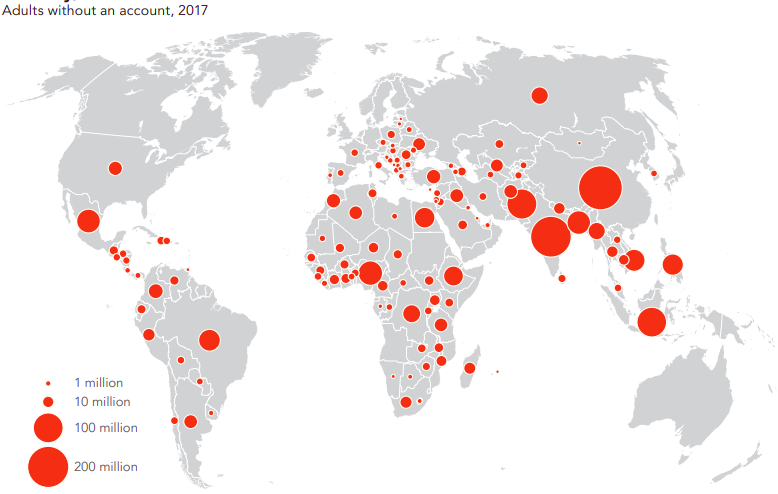
\includegraphics[height=4.2cm]{figs/unbanked_map.jpg}
        \vspace{1cm}
    \end{figure}
    \end{minipage}
\end{frame}

\begin{frame}{Introduction: Proven benefits}
    \begin{itemize}
        \item{Norwegian Refugee Council - Niger experiment}
        \begin{itemize}
            \item 5 Month relief program - swap from monthly cash payment to mobile
            \item Saved 20 hours in travel and wait time
        \end{itemize}
        \item{Norwegian Refugee Council - Kenya experiment}
        \begin{itemize}
            \item Similar study in Kenya
            \item 20\% increased savings
        \end{itemize}
    \end{itemize}
\end{frame}

\begin{frame}{Introduction: Financially included regions}
    \vspace{.5cm}
    \begin{table}[!ht]
    \begin{tabular}{|l|l|l|l|}
    \hline
    \textbf{Region}       & \textbf{Account (\%)} & \textbf{FI\footnote{Financial institution account}(\%)} & \textbf{M\footnote{Mobile money account} (\%)} \\ \hline
    East Asia \& Pacific    & 70.6          & 70.3           & 1.3                \\ \hline
    Europe \& Central Asia    & 65.3          & 65.1           & 3.2                \\ \hline
    Latin American \& Caribbean & 54.4          & 53.5           & 5.3                \\ \hline
    The Middle East \& North Africa & 43.5          & 43.0           & 5.8                \\ \hline
    South Asia          & 69.6          & 68.4           & 4.2                \\ \hline
    Sub-Saharan Africa      & 42.6          & 32.8           & 20.9                 \\ \hline
    \end{tabular}
    \caption{Financial inclusion statistics from six regions of the world, aged 15 and up}.
    \label{tab:financial_statistics}
    \end{table}
\end{frame}

\begin{frame}{Introduction: Reasons}
    Common reasons for being financially excluded
    \vspace{.5cm}
        \begin{table}[!ht]
        \centering
        \begin{tabular}{|l|l|l|}
        \hline
        \textbf{Reason} & \textbf{SSA (\%)} & \textbf{MENA (\%)} \\ \hline
        Distance to bank & 19 & 5 \\ \hline
        Services are too expensive & 19 & 12 \\ \hline
        Lack of necessary documentation & 18 & 7 \\ \hline
        Lack of trust in financial institutions & 10 & 7 \\ \hline
        Religious reasons & 4 & 4 \\ \hline
        Insufficient funds & 51 & 44 \\ \hline
        A family member has an account & 8 & 7\\ \hline
        \end{tabular}
        \vspace{0.1cm}\caption{Reasons for lack of financial accounts in SSA and MENA}
        \label{tab:ssa_mena_reasons}
        \end{table}
\end{frame}

\begin{frame}{SSA: Determining the best suited country}
    \vspace{.5cm}
    \begin{itemize}
        \item Example-driven approach
        \item Contributing factors
        \begin{itemize}
            \item Country specifics (e.g. mobile penetration rate)
            \item Financial specifics (e.g. financial inclusion rate)
            \item Population specifics (e.g. literacy level)
        \end{itemize}
    \end{itemize}
\end{frame}

\begin{frame}{SSA: Determining the best suited country 2}
    \vspace{.5cm}
    Filtering by financial inclusion rate

    \begin{table}[!ht]
    \centering
    \begin{tabular}{|l|l|l|l|}
    \hline
    \textbf{Country}        & \textbf{M (\%)} & \textbf{FI (\%)} & \textbf{F. Inclusion (\%)} \\ \hline
    Burundi             & 0.7            & 7.0                      & 7.0                  \\ \hline
    Central African Republic    & 0.0            & 13.7                       & 13.7                  \\ \hline
    Chad              & 15.2             & 8.8                      & 21.8                 \\ \hline
    Congo, Democratic Republic of & 16.1             & 15.0                       & 25.8                  \\ \hline
    Ethiopia            & 0.3            & 34.8                       & 34.8                  \\ \hline
    Guinea            & 13.8             & 14.6                       & 23.5                  \\ \hline
    Madagascar          & 12.1             & 9.6                      & 17.9                  \\ \hline
    Mauritania          & 4.0            & 19.0                       & 20.9                  \\ \hline
    Niger             & 8.7            & 9.5                      & 15.5                  \\ \hline
    Sierra Leone          & 11.0             & 12.4                       & 19.8                  \\ \hline
    South Sudan           & 0.0            & 8.6                      & 8.6                  \\ \hline
    \end{tabular}
    \vspace{0.1cm}\caption{Financial inclusion statistics for some of the 11 most financially excluded countries in SSA.}
    \end{table}
\end{frame}

\begin{frame}{SSA: Determining the best suited country 3}
    \vspace{.4cm}
    Filtering by mobile penetration rate

\begin{table}[ht]
\centering
\begin{tabular}{|l|l|l|l|}
\hline
\textbf{Country}        & \textbf{Mobile (\%)} & \textbf{Internet (\%)} \\ \hline
Burundi             & 56.65             & 2.66                                        \\ \hline
Central African Republic    & 33.62             & 4.34                                      \\ \hline
Chad              & 48.07             & 6.5                                       \\ \hline
Congo, Democratic Republic of & 42.77             & 8.62                                       \\ \hline
Ethiopia            & 37.22             & 18.62                                       \\ \hline
Guinea            & 100.8             & 21.83                                       \\ \hline
Madagascar          & 40.57             & 4.71                                        \\ \hline
Mauritania          & 104.09            & 20.8                                       \\ \hline
Niger             & 40.64             & 5.25                                        \\ \hline
Sierra Leone          & 86.13             & 13.24                                       \\ \hline
South Sudan           & 20.09             & 7.98                                        \\ \hline
\textbf{Average}        & \textbf{55.51}        & \textbf{10.41}                                        \\ \hline
\end{tabular}
\vspace{0.1cm}\caption{Mobile and internet penetration in SSA for some of the 11 most financially excluded countries in SSA.}
\end{table}
\end{frame}

\begin{frame}{SSA: Determining the best suited country 4}
    \vspace{.5cm}
    \textbf{Burundi}
    \begin{itemize}
        \item Poor: \$261.2 GDP per capita
        \item 90\% work in agriculture for subsistence
    \end{itemize}
    \textbf{Guinea}
    \begin{itemize}
        \item Decent economy: \$962.8 GDP per capita
        \item Over 100\% mobile phone penetration rate
        \item Highest internet penetration rate (21.83\%)
    \end{itemize}
    \textbf{Mauritania}
    \begin{itemize}
        \item Rich economy: \$1,679.4
        \item Lists few reasons to needing a bank
    \end{itemize}
    \textbf{Sierra Leone}
    \begin{itemize}
        \item Poor: \$527.5 GDP per capita
        \item Recovering from civil war
        \item More mobile banks than traditional banks
    \end{itemize}
\end{frame}

\begin{frame}{Guinea}
\begin{itemize}
\item Dense population (51.94 p/km²)
\item 2.6 average years of schooling
\item 30\% literacy level
\item 30\% financially literate
\item Multiple languages
\end{itemize}
\end{frame}

\begin{frame}{Guinea: Reasons}
\begin{table}[!ht]
\centering
\begin{tabular}{|l|l|l|l|}
\hline
\textbf{Reason} & \textbf{Guinea (\%)} \\ \hline
Distance to bank & 30\\ \hline
Services are too expensive & 30 \\ \hline
Lack of necessary documentation & 38 \\ \hline
Lack of trust in financial institutions & 15 \\ \hline
Religious reasons & 11 \\ \hline
Insufficient funds & 74 \\ \hline
A family member has an account & 8\\ \hline
\end{tabular}
\vspace{0.1cm}\caption{Reasons for lack of financial accounts in Guinea}
\end{table}
\end{frame}

\begin{frame}{Guinea: Existing banks}
\begin{itemize}
    \item 23.5\% are financially included
    \item 14.6\% partake in mobile banking
\end{itemize}
\vspace{0.4cm}
Existing competitors:

\begin{itemize}
    \item Orange Money
    \item MTN Mobile Money
\end{itemize}

\vspace{0.4cm}
Agent-based model
\begin{itemize}
\item USSD
\item Use local licened shops
\item Upfront capital
\item Shop-owner has a large role
\item Higher risk of robberies
\end{itemize}

\end{frame}


\begin{frame}{Product: Requirements}
\begin{enumerate}
    \item Different/cheaper than existing competitors
    \item Simple
    \item Mobile-phone based
    \item Widely available
    \item Cheap
    \item Ideally be available to the unidentifiable
    \item Support french or the larger languages
    \item Allow for easy transition from cash to online payment
    \item Single player mode
\end{enumerate}
\end{frame}

\begin{frame}{Product: Description}
\begin{wideitemize}
    \item Two implementations
    \begin{itemize}
        \item USSD
        \item Android
    \end{itemize}
    \item Agent-based
    \begin{itemize}
        \item Swap from businesses to local citizens
    \end{itemize}
\end{wideitemize}
\end{frame}

\begin{frame}{Product: Features}
\begin{itemize}
    \item Transfer money
    \item Request money
    \item Deposit money
    \item Withdraw money
    \item View transaction history
    \item Confirm pending transactions
    \item Decline pending transactions
    \item View balance
    \item Enable/Disable agent status
    \item Request help
    \item Register account
\end{itemize}
\end{frame}

\begin{frame}{Demo}
\textbf{Demo}
\end{frame}

\definecolor{yel}{RGB}{213, 191, 29}
\definecolor{gre}{RGB}{0, 195, 49}


\begin{frame}{Conclusion}
\begin{enumerate}
    \item {\color{yel} (\checkmark)} Different/cheaper than existing competitors
    \item {\color{gre} \checkmark} \ \ Simple
    \item {\color{gre} \checkmark} \ \ Mobile-phone based
    \item {\color{yel} (\checkmark)} Widely available
    \item {\color{yel} (\checkmark)} Cheap
    \item {\color{yel} (\checkmark)} Ideally be available to the unidentifiable
    \item {\color{gre} \checkmark} \ \ Support french or the larger languages
    \item {\color{gre} \checkmark} \ \ Allow for easy transition from cash to online payment
    \item {\color{red} X } \ \ Single player mode
\end{enumerate}
\end{frame}

\begin{frame}{Questions}
\textbf{Questions}
\begin{figure}
        \centering
        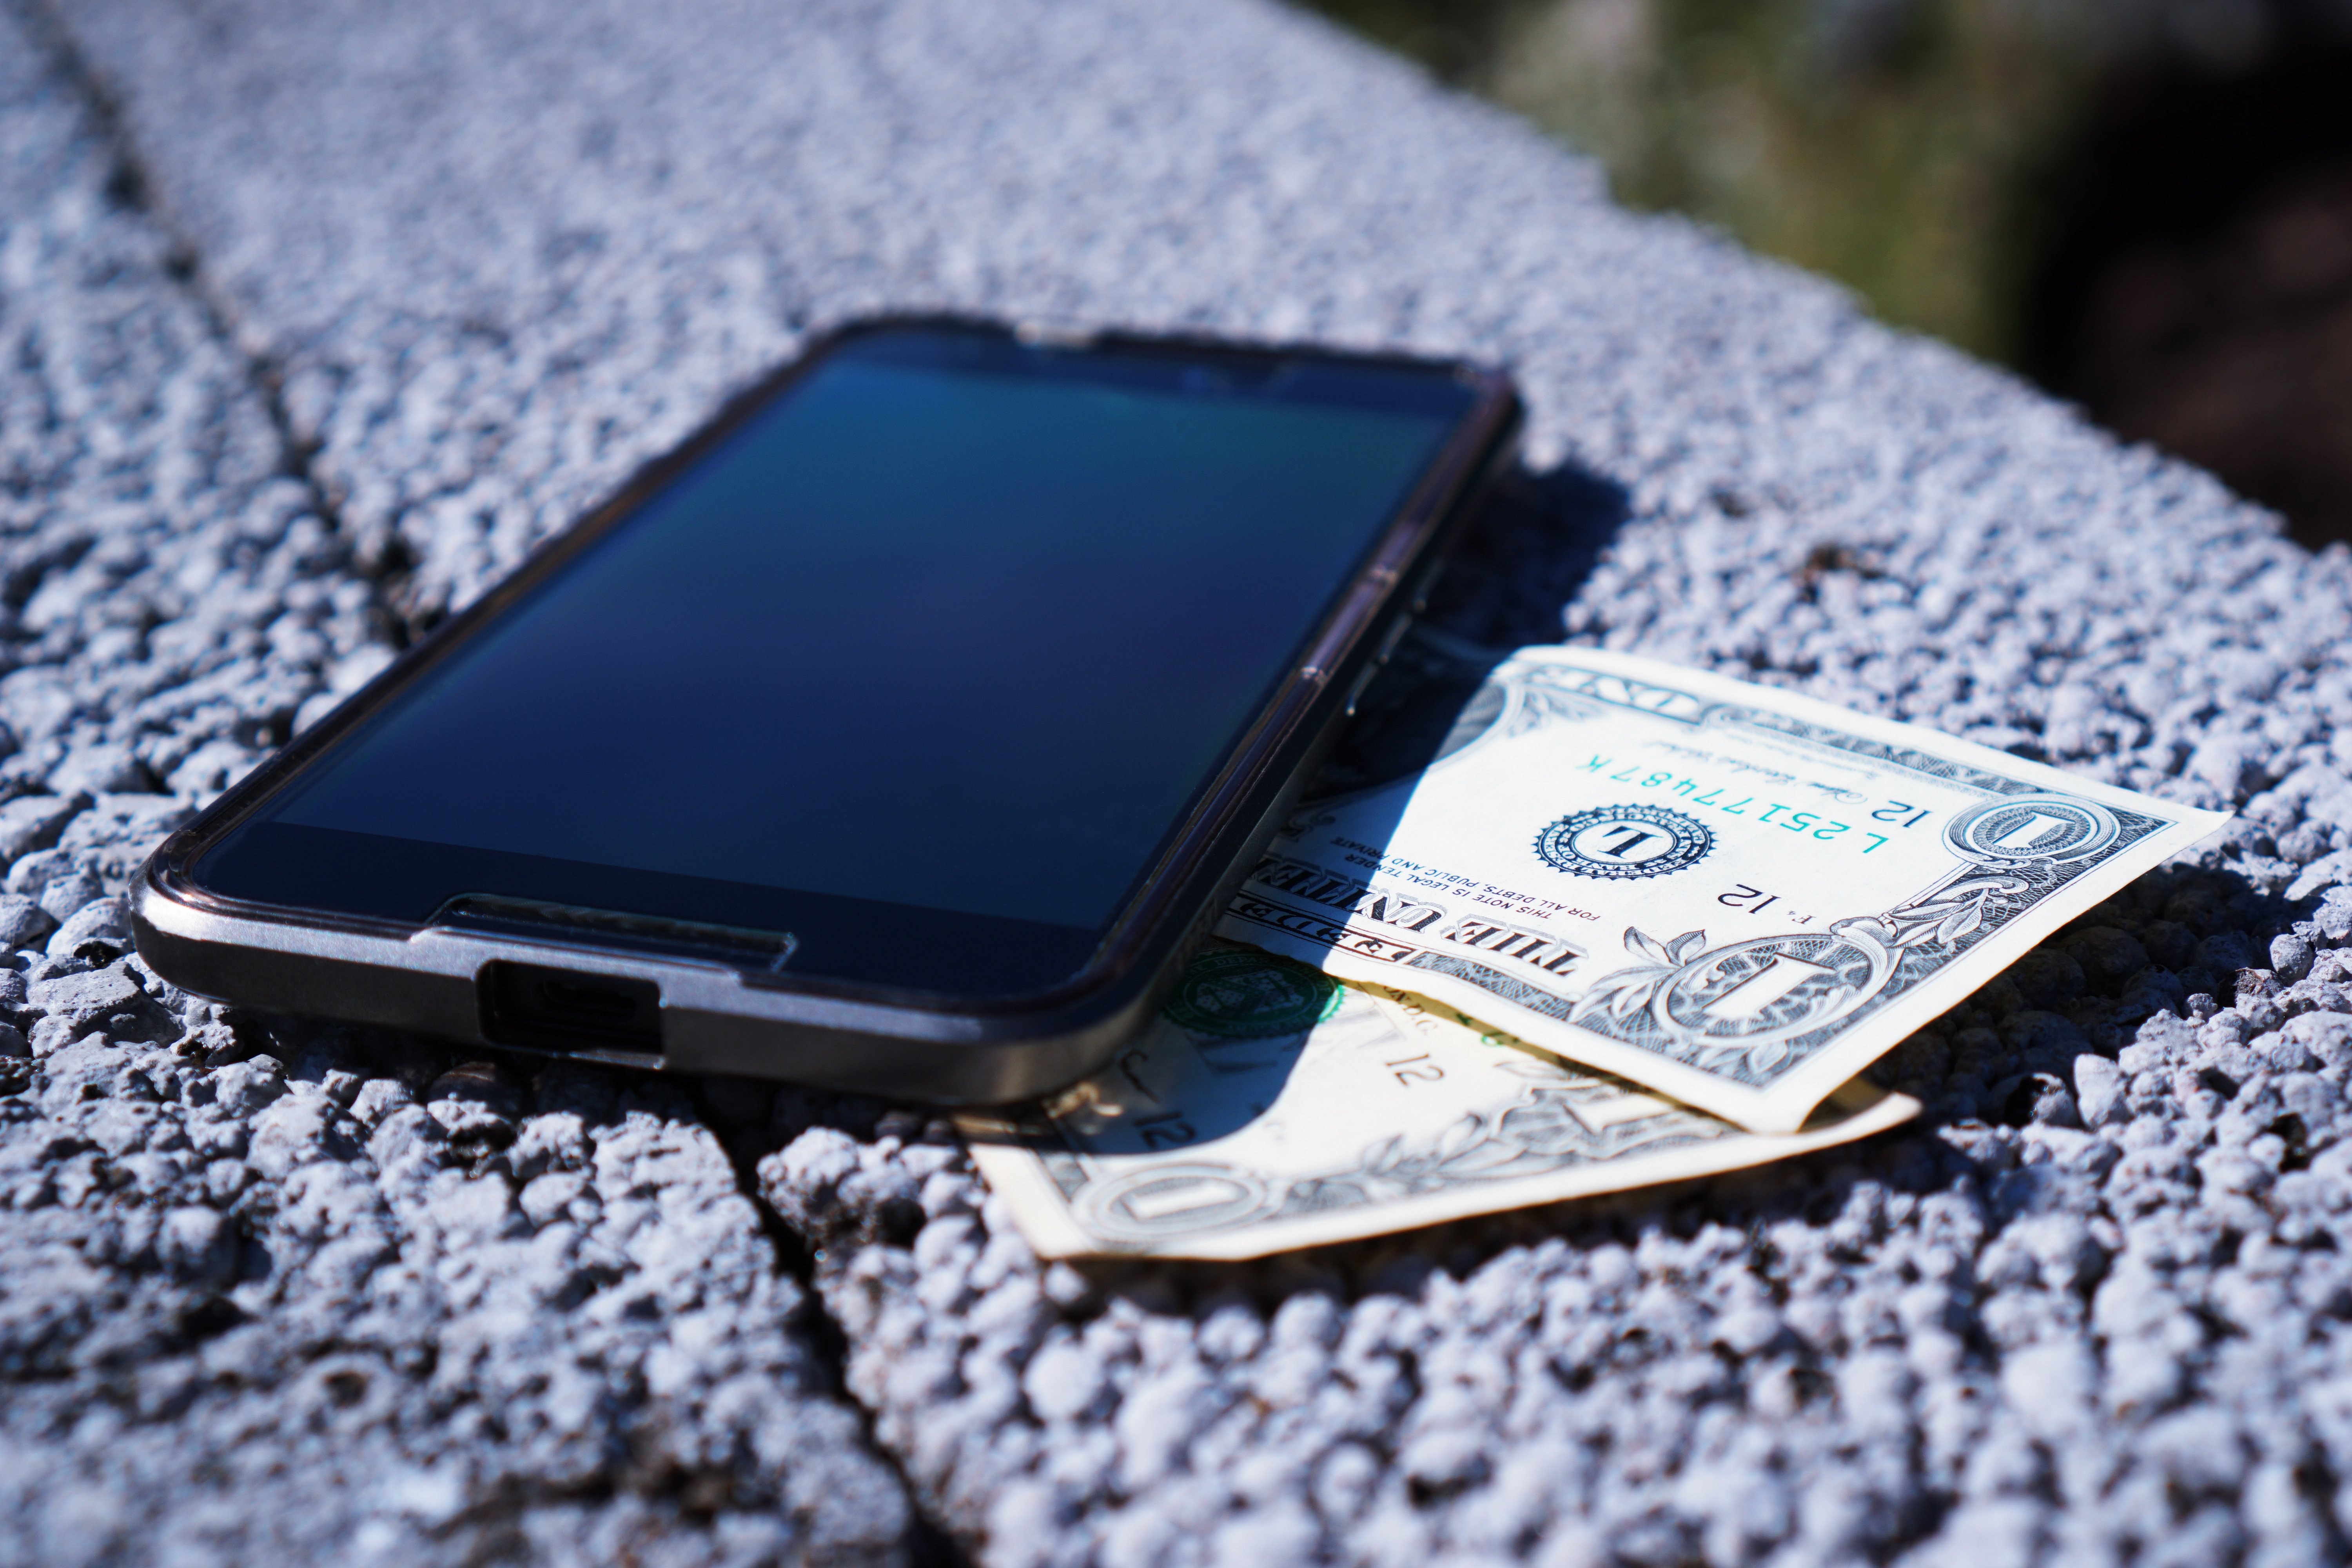
\includegraphics[height=5.2cm]{figs/phonecashheader.jpg}
        \vspace{1cm}
    \end{figure}
\end{frame}


\end{document}
